%
% problemtypen.tex -- Anfangs- und Endbedingungen
%
% (c) 2021 Prof Dr Andreas Müller, OST Ostschweizer Fachhochschule
%
\bgroup
\begin{frame}[t]
\setlength{\abovedisplayskip}{5pt}
\setlength{\belowdisplayskip}{5pt}
\frametitle{Problemtypen}
\vspace{-10pt}
\begin{center}
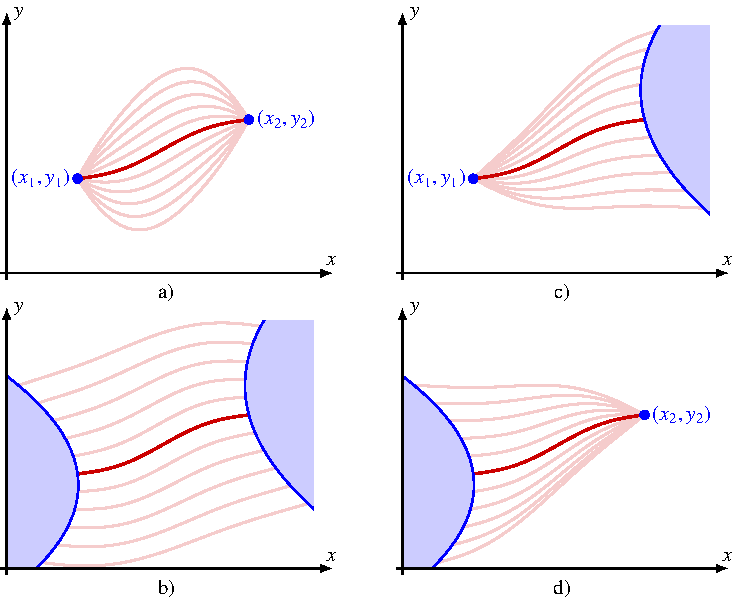
\includegraphics[width=0.7\textwidth]{../../buch/chapters/020-variation/images/grundaufgaben.pdf}
\end{center}
\end{frame}
\egroup
